\documentclass[12pt]{article}
\usepackage{graphicx}
\usepackage[usenames,dvipsnames]{xcolor}
\usepackage{color}
\usepackage[ utf8]{inputenc} %Codificación
\usepackage[activeacute,spanish]{babel} %Para escribir en español y con tildes ej: eón y no e\'on

%codigos: \begin{abstract} \end{abstract} es resumen
%nueva pagina \newpage
%colores predefinidos : white, black, red, green, blue, cyan, magenta, yellow
%\textcolor{blue}{text}
%\color{blue!20!black!30!green}{Prueba} mezcla de colores, conviene manejar solo 2 colores, es mas manejable

\title{{\LARGE \textbf{\color{blue}{MY TWIN}}}}
\author{Kevin M. Calder\'on\\C\'esar E. SanLucas\\Hern\'an R. Ull\'on}
\date{}

\begin{document}
\maketitle

%\begin{figure}[h]
%\centering
%\includegraphics[scale=0.5]{Hao}     % comentario de figuras, parte del logo
%\end{figure}
%\includegraphics[totalheight=1.2in,width=1in]{Hao}

\newpage
\section{Introducción} 

\textbf{MY TWIN} es una aplicación dirigida a toda clase de usuario mediante la cual podrás crear tu propio avatar usando una fotografía de tu rostro por aquello el nombre My Twin, el cual se convertirá en tu asesor personal y virtual de tareas de una manera mucho más agradable. 

Una aplicación la cual jugará con los estados de ánimo de tu avatar, los cuales estarán definidos por las diferentes tareas que cumplirá. Esto es que la aplicación no solo será para entretenimiento tendrá una funcionalidad que buscará ayudar al usuario de una manera diferente, entretenida y personalizada.\\
\subsection{Tareas} 

\hspace{0.2in}*BATERÍA: El TWIN  nos  mostrará el estado de la batería, indicándonos si se encuentra cargada o por descargarse y necesita necesariamente ser recargada, mediante mensajes de voz, acompañado de cambios de ánimo de nuestro avatar, esto es, si se encuentra la batería cargada el avatar se mostrará contento, del mismo modo si ocurre lo contrario, el ánimo del avatar también se verá afectado negativamente\\. 

\hspace{0.2in}*RECORDATORIOS: Nos ayudará a recordar las fechas importates tales como cumpleaños o aniversarios, mostrándose el avatar en una imagen de acuerdo al evento a recordar en el cual nos indicará el acontecimiento y hora del mismo, de un modo poco usual y entretenido, haciendo así que sea mas fácil de tener en mente todo el día aquel acontecimiento importante (Ideal si se nos ha olvidado comprar un regalo)\\. 

\hspace{0.2in}*AYUDA PERSONALIZADA: Nuestro TWIN estará para recordarnos todo lo que tengamos planeados, a la hora precisa para realizar lo que tengamos planeado, también nos indicará cuando no hemos hecho algo que debimos hacer, todo lo hará interactuando con el usuario de un modo personalizado, porque lo hará con nuestra imagen, nuestra voz y con estados de ánimo con el que fácilmente comprenderemos lo que nos quiere transmitir.

\newpage
\section{Descripción}

\subsection{Divertido}
La aplicación de MY TWIN será una manera divertida de recibir ayuda por tu celular y por ti mismo... Es decir por el TWIN.
Pero ¿Qué hace que este ayudante sea divertido, novedoso y que pueda ayudarnos a la vez?
La aplicación tendrá una presentación similar a la de un juego, de hecho, el personalizar a nuestro TWIN, puede resultar siendo parte de un juego para el usuario; se tendrá la opción de personalizar eligiendo de diversas plantillas de cuerpo disponible del avatar a nuestro gusto con el único objetivo es que sea lo mas semejante al usuario, utilizando recursos que nos brinda nuestro teléfono; finalmente, aquel personaje al que dimos vida, pasará a ayudarnos cada vez que sea necesario, llevando el beneficio de tener a nuestro lado o más bien en nuestro bolsillo a alguien que nos ayude y ¿Quién mas confiable que nuestro TWIN?.

\subsection{Realista}
La intención es de tener una aplicación realista, amigable con el usuario y a la vez tan real como para ser una aplicación de gran importancia en nuestro dispositivo móvil, ya que ha sido pensado para brindar una ayuda sencilla y eficaz ante simples pero importantes necesidades que podemos ver en la vida cotidiana como recordar el cumpleaños de un amigo o amiga que estimemos mucho que por algún motivo hayamos olvidado, recordar realizar una tarea o entregar algún proyecto en la fecha adecua o hasta recordarnos una reunion muy importante en el ámbito laboral o social.

\newpage
\section{Fucionamiento General del Twin}

\subsection{Creaci\'on del Avatar}
Este es el primer paso que daremos luego de descargar e instalar la aplicaci\'on en nuestro dispositivo m\'ovil. La primera pantalla que veremos nos indicar\'a por medio de unos emoticones el tipo de foto que debemos tomarnos para que le vayamos dando vida a nuestro avatar. Debajo del dibujo de caras (Feliz, Triste, Enojado), se encontrar\'a el dibujo de una c\'amara, al presionar en la figura pasaremos a tomar la foto que corresponde.\\
Luego de completar eso podremos avanzar presionando en el visto. 

\begin{figure}[h]
\centering
\vspace{0.3in}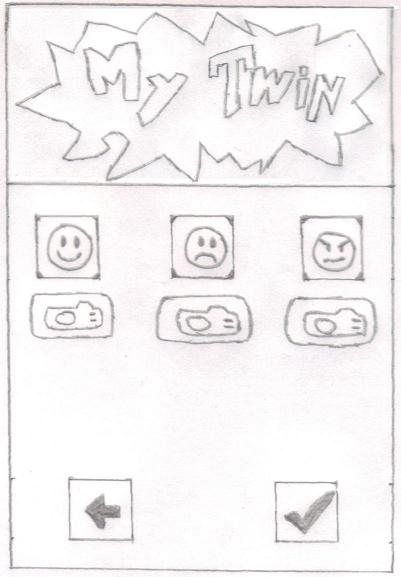
\includegraphics[scale=0.5]{Twin1}
\end{figure}

\newpage
\subsubsection{Elecci\'on del cuerpo del Avatar}
Esta es una opci\'on mas de personalizaci\'on, porque podremos escoger el cuerpo que tendr\'a el TWIN de entre algunos ya precargados, podremos realizar nuestra elecci\'on ya sea a nuestro gusto o porque veamos que es la que mas se ajusta a nuestra personalidad. 
Si no nos sentiamos satisfechos con las imagenes que tomamos del paso anterior, tendremos la opci\'on de volver presionando en atr\'as, luego de seleccionar el modelo del cuerpo que queremos, solamente seleccionamos siguiente y habremos terminado.

\begin{figure}[h]
\centering
\vspace{0.3in}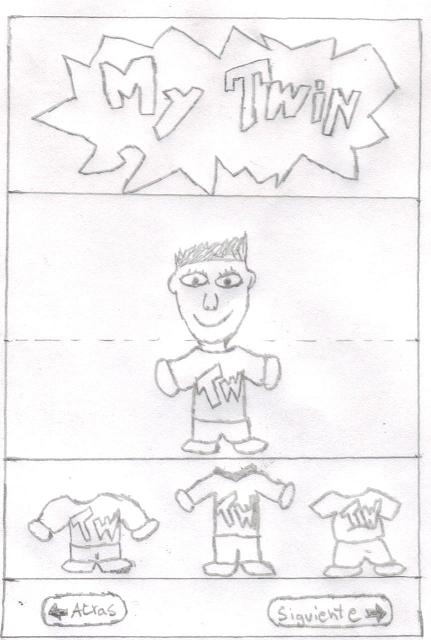
\includegraphics[scale=0.5]{Twin2}
\end{figure}
%\begin{figure}[h]
%\centering
%\includegraphics[totalheight=2in,width=2.5in]{CVPicture}\\\vspace{0.1in}  %figuras extras para parte explicativa
%\includegraphics[totalheight=2in,width=2.5in]{Hao}
%\end{figure}

\end{document}